%%%%%%%%%%%%%%%%%%%%%%%%%%%%%%%%%%%%%%%%%%%%%%%%%%%%%%%%%%%%%%%%%%%
%                                                                 %
%                            ROOT FILE                            %
%                                                                 %
%%%%%%%%%%%%%%%%%%%%%%%%%%%%%%%%%%%%%%%%%%%%%%%%%%%%%%%%%%%%%%%%%%% 
%
%  Run LaTeX or pdfLaTeX on this file to produce your dissertation.
%  To produce the abstract title page followed by the abstract,
%  see the file abstitle-phd.tex or abstitle-mas.tex.
%
%%%%%%%%%%%%%%%%%%%%%%%%%%%%%%%%%%%%%%%%%%%%%%%%%%%%%%%%%%%%%%%%%%%

\documentclass[chap,letterpaper]{thesis}
%%%%%%%%
\usepackage{epsfig, amssymb, amsmath, latexsym, graphicx, url}
\usepackage{color}    %Latex picture produced by xfig uses color
\usepackage{fancyhdr} %must be used with the chap option of the thesis class.
%\usepackage[square, comma]{natbib}  %the sample bibliography doesn't work with this.
\usepackage[toc, acronym]{glossaries}
%
% Research and use other cool Latex packages!
%

% yc added
\usepackage[colorlinks,citecolor=blue,urlcolor=blue,bookmarks=false,hypertexnames=true]{hyperref} 
\usepackage{lineno}
\usepackage{natbib}
\usepackage{siunitx}
\usepackage{graphicx}
\usepackage{float}
\usepackage{chngcntr}
\counterwithout{figure}{chapter}
\renewcommand{\baselinestretch}{1.8}
\setcitestyle{authoryear,open={},close={}}
\linenumbers
\graphicspath{{./img/}}

%%%%%%%% We determine text size and margin, not the style class file.
\setlength{\textheight}{9.0in} %to leave 1in top and bot margin
\setlength{\textwidth}{6.5in}  %to leave 1in left and right margin
\setlength{\topmargin}{-0.5in}
\setlength{\headheight}{0.5in}
\setlength{\headsep}{0.0in}
\setlength{\parskip}{0.5em}
\setlength{\oddsidemargin}{0.0in}  %to get a total of 1in
\setlength{\evensidemargin}{0.in}  %to get a total of 1in
\setlength{\footskip}{0.5in}

%%%% various custom math, etc added commands.  Try, edit, remove, replace as you wish
\newcommand{\ignore}[1]{}
\newcommand{\undr}{\underline}
\newcommand{\ovr}{\overline}
\newcommand{\flr}{\rightarrow}
\newcommand{\fll}{\leftarrow}
\newcommand{\fflr}{\longrightarrow}
\newcommand{\fl}{-\!\!\!-\!\!\!-\!\!\!-\!\!\!-\!\!\!}
\newcommand{\ffflr}{\fl\fflr}
\newcommand{\lft}{\noindent}
\newcommand{\Flr}{\Longrightarrow}
\newcommand{\mFlr}{\,{|}\!\!\!\Flr}
\newcommand{\app}{\approx}
\newcommand{\nat}{\mathbb{N}}

\newcommand{\proof}{{\em Proof\/}: }
\newcommand{\qed}{\hfill $\fbox{}$}

\newcommand{\disp}[1]{\vspace{-0.5em}\begin{center} {#1}
                                   \end{center}\vspace{-0.5em}}
\newcommand{\dispn}[2]{ {\noindent{#1}} \centerline{#2} }

\newcommand{\msup}[2]{\stackrel{#2}{#1}}

\newcommand{\h}{\bf h}

\newcommand{\A}{\bf A}
\newcommand{\B}{\cal B}
\newcommand{\C}{{\cal C}}
\newcommand{\D}{{\cal D}}
\newcommand{\E}{{\cal E}}
\newcommand{\F}{{\cal F}}
\newcommand{\m}{{\cal L}}
\newcommand{\M}{{\cal M}}
\newcommand{\s}{{\cal S}}
\newcommand{\U}{{\cal U}}
\newcommand{\W}{{\cal I}}

\newcommand{\G}{\mathcal{G}}
\newcommand{\I}{\mathcal{I}}
\renewcommand{\L}{\mathcal{L}}
\renewcommand{\P}{\mathcal{P}}
\newcommand{\Q}{\mathcal{Q}}
\newcommand{\R}{\mathcal{R}}
\renewcommand{\S}{\mathcal{S}}
\newcommand{\T}{\mathcal{T}}
\newcommand{\X}{\mathcal{X}}
\newcommand{\cc}{{\succ\!\!\!\succ}}

\newtheorem{theorem}{Theorem}[chapter]

\newtheorem{propn}{Proposition}[chapter]
\newtheorem{defn}{Definition}[chapter]
\newtheorem{corol}{Corollary}[chapter]
\newtheorem{lemma}{Lemma}[chapter]

\newcommand{\hsp}{\hspace*{0.7cm}}
\newcommand{\hsps}{\hspace*{1em}}
\newcommand{\hspa}{\hspace*{1cm}}
\newcommand{\hspb}{\hspace*{1.5cm}}
\newcommand{\donno}{\,?\,}

%%%%%%%%%%%%%%%%%%%%%%%%% Title Info %%%%%%%%%%%%%%%%%%%%%%%%%
% You should replace the appropriate fields in 
% the following section with your own information.

\thesistitle{\bf Research Prospectus}
\thesissubtitle{\bf The importance of ice microphysics on storm electrification}        
\author{Yichen Cai}        
\degree{Doctor of Philosophy}        
\college{College of Arts and Sciences}
\department{Department of Atmospheric and Environmental Sciences} 
\submitdate{}
% \submitdate{(Winter, Spring, Summer, Fall) 20xx or
%   (January, May, August, December) 20xx or 20xx}        
%\copyrightyear{1970}   % if omitted, current year is used.
\dedicatedto{To my}

% Committee info is not use at this time
%\signaturelines{3}     %max number of signature lines is 7        
%\thadviser{My Advisor}
%\cothadviser{Second Adviser} % If you have 2 thesis advisers
%\memberone{My Committee Member}        
%\membertwo{My Other Committee Member}
%\memberthree{Aristotle}
%\memberfour,\memberfive, \membersix        
% can also be used. Remember to change \signaturelines.%
%%%%%%%%%%%%%%%%%%%%%%%% End Title Info %%%%%%%%%%%%%%%%%%%%%%%%%

%%Glossary.  This command and the glossary entries must go in the preamble,
%% so you must \input (NOT \include) 
\makeglossaries
\makeglossaries

\newglossaryentry{eregex}{name={eregex},
description={An extended regular expression, i.e. a regular expression with the addition of backreferences}}

\newacronym{SRE}{SRE}{Synchronized Regular Expression}

  

%\includeonly{chapter1}  % When computers were slower, we used \includeonly to process only
                         % the file(s) listed inside the braces                       
\begin{document}
 
\titlepage     
% \dedication   %optional

% %%%%%%%%%%%%%%%%%%%%%%%%%%%%%%%%%%%%%%%%%%%%%%%%%%%%%%%%%%%%%%%%%%% 
%                                                                 %
%                            ABSTRACT                             %
%                                                                 %
%%%%%%%%%%%%%%%%%%%%%%%%%%%%%%%%%%%%%%%%%%%%%%%%%%%%%%%%%%%%%%%%%%% 
 
\specialhead{ABSTRACT}

Enter your abstract here.  %The heading for abstract, acknowledgment, introduction, chapter, etc.
% %%%%%%%%%%%%%%%%%%%%%%%%%%%%%%%%%%%%%%%%%%%%%%%%%%%%%%%%%%%%%%%%%%% 
%                                                                 %
%                         ACKNOWLEDGEMENT                         %
%                                                                 %
%%%%%%%%%%%%%%%%%%%%%%%%%%%%%%%%%%%%%%%%%%%%%%%%%%%%%%%%%%%%%%%%%%% 
 
\specialhead{ACKNOWLEDGMENT}

%---------------------------------------------------------------------------------------%

I would like to thank...

I would also like to thank...

Finally, I would like to thank...

$M^2$
%is put in the included file, followed by the content.

\tableofcontents

% %%%%%%%%%%%%%%%%%%%%%%%%%%%%%%%%%%%%%%%%%%%%%%%%%%%%%%%%%%%%%%%%%%% 
%                                                                 %
%                            INTRODUCTION                         %
%                                                                 %
%%%%%%%%%%%%%%%%%%%%%%%%%%%%%%%%%%%%%%%%%%%%%%%%%%%%%%%%%%%%%%%%%%% 
 
\chapter{Introduction}

%---------------------------------------------------------------------------------------%

Enter your introduction here.


Lines of lines of sample text and lots of sample text many many lines
of it are hear repeated and repeated and repeated for all times and days
and months for me to read.  Lots and lots of sample text for you to
see how it fits into the document and make sure it looks good and
tells the academic truths for all to read.  More and more and more
before it all ends. A picture is worth 1000 words.

\begin{figure}
  \begin{center}
    \input{drawline.pdf_t}
  \end{center}
  \caption{A Line and a segment thereof.}
\end{figure}


Lines of lines of sample text and lots of sample text many many lines
of it are hear repeated and repeated and repeated for all times and days
and months for me to read.  Lots and lots of sample text for you to
see how it fits into the document and make sure it looks good and
tells the academic truths for all to read.  More and more and more
before it all ends.  

Lines of lines of sample text and lots of sample text many many lines
of it are hear repeated and repeated and repeated for all times and days
and months for me to read.  Lots and lots of sample text for you to
see how it fits into the document and make sure it looks good and
tells the academic truths for all to read.  More and more and more
before it all ends.  

Lines of lines of sample text and lots of sample text many many lines
of it are hear repeated and repeated and repeated for all times and days
and months for me to read.  Lots and lots of sample text for you to
see how it fits into the document and make sure it looks good and
tells the academic truths for all to read.  More and more and more
before it all ends.  

Lines of lines of sample text and lots of sample text many many lines
of it are hear repeated and repeated and repeated for all times and days
and months for me to read.  Lots and lots of sample text for you to
see how it fits into the document and make sure it looks good and
tells the academic truths for all to read.  More and more and more
before it all ends.  

Lines of lines of sample text and lots of sample text many many lines
of it are hear repeated and repeated and repeated for all times and days
and months for me to read.  Lots and lots of sample text for you to
see how it fits into the document and make sure it looks good and
tells the academic truths for all to read.  More and more and more
before it all ends.  

Lines of lines of sample text and lots of sample text many many lines
of it are hear repeated and repeated and repeated for all times and days
and months for me to read.  Lots and lots of sample text for you to
see how it fits into the document and make sure it looks good and
tells the academic truths for all to read.  More and more and more
before it all ends.  

Lines of lines of sample text and lots of sample text many many lines
of it are hear repeated and repeated and repeated for all times and days
and months for me to read.  Lots and lots of sample text for you to
see how it fits into the document and make sure it looks good and
tells the academic truths for all to read.  More and more and more
before it all ends.  

Lines of lines of sample text and lots of sample text many many lines
of it are hear repeated and repeated and repeated for all times and days
and months for me to read.  Lots and lots of sample text for you to
see how it fits into the document and make sure it looks good and
tells the academic truths for all to read.  More and more and more
before it all ends.  

Lines of lines of sample text and lots of sample text many many lines
of it are hear repeated and repeated and repeated for all times and days
and months for me to read.  Lots and lots of sample text for you to
see how it fits into the document and make sure it looks good and
tells the academic truths for all to read.  More and more and more
before it all ends.  

Lines of lines of sample text and lots of sample text many many lines
of it are hear repeated and repeated and repeated for all times and days
and months for me to read.  Lots and lots of sample text for you to
see how it fits into the document and make sure it looks good and
tells the academic truths for all to read.  More and more and more
before it all ends.  

Lines of lines of sample text and lots of sample text many many lines
of it are hear repeated and repeated and repeated for all times and days
and months for me to read.  Lots and lots of sample text for you to
see how it fits into the document and make sure it looks good and
tells the academic truths for all to read.  More and more and more
before it all ends.  

Lines of lines of sample text and lots of sample text many many lines
of it are hear repeated and repeated and repeated for all times and days
and months for me to read.  Lots and lots of sample text for you to
see how it fits into the document and make sure it looks good and
tells the academic truths for all to read.  More and more and more
before it all ends.  





%%%%%%%%%%%%%%%%%%%%%%%%%%%%%%%%%%%%%%%%%%%%%%%%%%%%%%%%%%%%%%%%%%% 
%                                                                 %
%                            CHAPTER                              %
%                                                                 %
%%%%%%%%%%%%%%%%%%%%%%%%%%%%%%%%%%%%%%%%%%%%%%%%%%%%%%%%%%%%%%%%%%% 
 
\chapter{Chapter Title}
\resetfootnote %this command starts footnote numbering with 1 again.

%---------------------------------------------------------------------------------------%
\section{Section One Title}
%---------------------------------------------------------------------------------------%

Here is a file for your chapters.  Copy this file for each chapter 
and change the titles.  Don't forget to add include statemets to 
dissertation.tex.  
You can use sections (as above).  
You can add glossary terms like \gls{eregex} and acronyms like \glsname{SRE}.
You can use footnotes.\footnote{Here is a footnote.}
Don't forget to cite books~\cite{Sipser} and papers~\cite{CarleNarendran}.

%---------------------------------------------------------------------------------------%
\section{Section Two Title}
%---------------------------------------------------------------------------------------%

Here is the content for section two.

%%%%%%%%%%%%%%%%%%%%%%%%%%%%%%%%%%%%%%%%%%%%%%%%%%%%%%%%%%%%%%%%%%% 
%                                                                 %
%                            CHAPTER                              %
%                                                                 %
%%%%%%%%%%%%%%%%%%%%%%%%%%%%%%%%%%%%%%%%%%%%%%%%%%%%%%%%%%%%%%%%%%% 
 
\chapter{Background}
\resetfootnote %this command starts footnote numbering with 1 again.

The vast majority of lightning occurs in cold/mixed phased clouds (\cite{wallace2006atmospheric}), where the interaction of ice phase hydrometeors is a fundamental ingredient for lightning production. It is generally accepted that the electrical structure of thunderstorms is developed by updrafts that separate hydrometeors (ice \& graupel esp.) with opposite charge signs into upper and lower levels (\cite{saunders2008charge}). The transfer of electric charge results from collisions of hydrometeors, and is highly sensitive to thermodynamic conditions within which they are grown. In most severe thunderstorms associated with intense updrafts and thus large vertical extent, a sufficient frozen hydrometeor growth zone (above \SI{0}{\celsius} level) and the charge zone (0$\sim$\SI{-20}{\celsius}) are almost guaranteed. The large vertical span also provides colorful growth environments which culture hydrometeors of various properties. This variety is the fundamental reason for differed charge density on particle surface among hydrometeor types (e.g., pristine ice crystals, snow aggregates, graupel), and subsequently a transfer of charge upon particle collisions in an attempt to neutralize the charge imbalance. 

%---------------------------------------------------------------------------------------%
\section{Charging Mechanisms}
%---------------------------------------------------------------------------------------%
A question that scientists have attempted to answer since late 1800's: Exactly how is charge generated in the cloud? Countless mechanisms have been proposed. Lenard Effect (also called spray electrification) was first studied by \cite{lenard1892berdie} trying to explain charging of thundercloud by drop break-up process. But this process, as stated in \cite{saunders2008charge}, is too rare and unorganized to produce strong cloud charge structure. Ions, as introduced to the  atmosphere through cosmic rays and  ground radioactivity, has been believed to involve in cloud charging. \cite{wilson1929some} described a mechanism where falling particles acquire charge by capturing ions positioned in lower half of atmosphere due to fair weather electric field, but this mechanism was later determined to be insufficient to create electric breakdown. As the study of mesoscale storm dynamics progresses, \cite{grenet1947essai} and \cite{vonnegut1953possible} first connected the distribution of charge to storms' air motion. In their theory, positive ions on earth surface are brought to cloud top by updraft, while falling particles capture negative ions that are attracted to the cloud edge, establishing separated regions of opposite charge in cloud. However, the charging contributed by convective processes were examined to be weak and disorganized, in 3-D simulations of storm electrification in \cite{helsdon2002examination}. Later on, some mechanisms involving hydrometeor interaction (e.g., charging through freezing potential upon droplet-ice collision \cite{workman1950electrical}, charge transfer through contact potential \cite{caranti1980surface}, ice lattice dislocation that carries local positive charge \cite{keith1990further}, temperature difference between colliding ice particles \cite{latham1961generation}, charged ice splinters ejected upon freezing of supercooled liquid during Hallet-Mossop multiplication process \cite{hallett1979charge}), though proven to be insufficient to initiate lightning by self, all contributed to the development of more untenable charging mechanisms.

So far, two mechanisms are considered to have withstand the test of time: Inductive charging and Noninductive charging. Both two mechanisms are, in short, the charge separation that occurs upon the collision and rebound of two ice particles. 

Inductive charging requires a previously established electric field (initially a weak downward fair weather field), which vertically polarizes the ice particles within. When a larger particle (e.g., graupel) falls with larger fall speed, and collide into a smaller particle with smaller fall speed, the contact point is more likely to be at the lower half of the larger particle. Upon collision, the positive charge induced to the lower half of the larger particle transfer to the smaller particle. Then if rebounding, the smaller particle will carry net positive charge and be carried upward by the updraft, while the graupel precipitate to lower parts of the cloud. This charge separation then reinforces the ambient electric field, promoting more inductive charging. \cite{brooks1994experimental} carried out experiment in cloud chamber and showed significant charge transferred to an ice surface when falling through supercooled droplets. But the limitation of inductive charging mechanism remains since an observational study \cite{christian1980airborne} found that graupels could not be charged as much as what was observed, even with a maximum electric field measured in cloud. Inductive charging is considered the secondary charging mechanism that is only significant at later stages of the storm.

The non-inductive charging mechanism has been proposed and studied since late 1950s, and was, over time, accepted as the primary and initial mechanism for cloud charging. As can be inferred from its name, this mechanism does not require a background electric field that polarize ice particle vertically. Instead, scientists suggested an ice particle internal charge gradient that is inward-out, before collision occurs. The conceiving of this mechanism was inspired by some lab results \cite{takahashi1978riming} that the sign and magnitude of charge gained by graupel is dependent on ambient temperature and liquid water content. However, the lab results (e.g., \cite{takahashi1978riming}, \cite{saunders1998laboratory}, \cite{pereyra2000laboratory}, \cite{saunders2006laboratory}) of sign of charge transferred to graupel varied significantly, as shown in Fig \ref{fig:charge_reverse_curves} from \cite{saunders2008charge}. Proposed by \cite{baker1987influence}, the relative vapor diffusional growth (VDG) rate theory explained such variation. Based on Baker's results from their cold room, the current flowing to the graupel is negative when colliding ice crystals grow faster than the graupel itself through vapor deposition, and is positive for the opposite. Riming is important in this mechanism given its modulation of graupel surface condition through 1) modulating VDG rate (by providing extra vapor to and heating of graupel surface); and 2) increasing the thickness of graupel's transitional layer, which affects the mass transfer upon collision. The variation of sign reversal curses derived from different cloud chambers can be accounted for by the different setup for the ice crystals growth environment right before their contact with rimers. A more turbulent cloud environment increases the likelihood of ice crystal experiencing a spike of growth rate immediately before collision, and thus negative charge being transferred to the graupel.
%---------------------------------------------------------------------------------------%
\section{Role of Ice Crystal Growth}
%---------------------------------------------------------------------------------------%

Here is the content for section two.

%---------------------------------------------------------------------------------------%
\section{Role of Riming}
%---------------------------------------------------------------------------------------%
%%%%%%%%%%%%%%%%%%%%%%%%%%%%%%%%%%%%%%%%%%%%%%%%%%%%%%%%%%%%%%%%%%% 
%                                                                 %
%                            CHAPTER                              %
%                                                                 %
%%%%%%%%%%%%%%%%%%%%%%%%%%%%%%%%%%%%%%%%%%%%%%%%%%%%%%%%%%%%%%%%%%% 
 
\chapter{Model Representation / Methodology}
\label{chap:models}
\resetfootnote %this command starts footnote numbering with 1 again.
A background on electrification and ice microphysics has been established, with a clear indication that the way in which ice particles are represented in numerical models could influence the prediction of lightning. Investigations of lightning using the Weather Research and Forecasting (WRF) model are facilitated by a modification to the framework to include computation of electrification, namely, WRF-ELEC (\href{https://sourceforge.net/projects/wrfelec/}{package} credits to Dr. Mansell, National Severe Storms Laboratory (NSSL)). In addition to the WRF-ELEC package, major amendments were incorporated in to the microphysical parameterization. Note that in this package, the simulated interaction between microphysics and charging is one-directional. That is, the computation of electrification is based on and fed by information of hydrometeors in the microphysics module; but results of electrification variables (e.g., particle charge, electric field, electric potential, lightning discharge) do not affect microphysical processes. 

Thus far, the WRF-ELEC package is only available in the National Severe Storm Laboratory Two-Moment (N2M) microphysics model (Mansell et al. 2010). More detailed microphysical models have since been developed, particularly for ice particle growth and subsequent collection (e.g., AHM). Given the sensitivity of electrification on ice hydrometeor interactions, an investigation into this sensitivity as a function of microphysical parameterization is warranted. And so, the purpose of this work is to implement the WRF-ELEC package into additional WRF microphysical modules to enable this analysis.

%---------------------------------------------------------------------------------------%
\section{N2M Model}

%---------------------------------------------------------------------------------------%
\subsection{Microphysics}
N2M is a fully two-moment bulk microphysics parameterization scheme, which predicts mass/number mixing ratio of cloud droplets, raindrops, ice crystals (columnar only), snow (including large ice crystals and aggregates), graupel and hail. Hydrometeors are assumed to have their size distributed in form of the gamma function, as stated in \cite{mansell2010simulated}: 
\begin{equation}
    N(v) = 
    A\frac{v^{\nu}}{\bar{v}^{\nu+1}}
    exp \left(
    -B{( \frac{v}{\bar{v}} )}^\mu
    \right)
    \label{eq:gamma_dis}
\end{equation}
where $N$ is number concentration of the species, $v$ is particle volume, $\nu,\mu$ are shape parameters specific to the particle category, and $A,B$ are functions of $\nu,\mu$ and their gamma function (see \cite{mansell2010simulated}). 
In the version available in this study, density of snow, graupel, and hail are prognostic and subject to change in total particle volume and the melting process: e.g., the density of graupel varies from 300 to 900 kg/m$^3$. The terminal fall velocity of graupel $V_g(D)$ is calculated based on diameter following \cite{schoenberg1994double}:
\begin{equation}
    V_g(D) = 
    (\frac{\rho_0}{\rho_{air}})^{1/2} a_g D^{b_g}
    \label{eq:graupel_fall}
\end{equation}
where $a_g$ and $b_g$ are fall speed parameters:
\begin{equation}
    a_g = \left(
    \frac{4\rho_g g} {3C_D\rho_{air}}
    \right)^{1/2}
    , b_g=\frac{1}{2}
\end{equation}
and $\rho_0,\rho_{air}$ are reference air density and actual air density, $D$ is graupel diameter. This calculation of fall speed is not capped with a maximal threshold, and has been found through initial sensitivity tests to reach values up to 78 m/s, which is not quite realistic. 

\subsection{Charging scheme}
\label{sec:n2m_charge}
The parameterization of electrification in WRF-ELEC is composed of charging and discharging components. The charging scheme in the N2M microphysics module prognostically calculates the change in charge density carried by all species of hydrometeors as well as ions (units of $Coulomb/kg$). These hydrometeor charge densities (HCDs) can evolve through the growth of the hydrometeors, as well as through hydrometeor interactions (e.g., collisions). These HCDs are then fed to and renewed by the discharge scheme outside the microphysics module, inside which the HCDs are used to compute electric field and electric potential, which are then used to parameterize lightning breakdown processes. Like other scalar variables, the HCDs are advected within the dynamic framework. Overall, the rate of change of the charge carried by a specific species is calculated by integrating the charge conservation equation (\cite{mansell2005charge}, equation 2), which considers
% \begin{equation}
%     \frac{\partial Q_n}{\partial t} = 
%     -\bm{\nabla}\cdot(\bm{V}Q_n)
%     +\bm{\nabla}\cdot(K_h\bm{\nabla} Q_n)
%     +\frac{\partial V_{T,n}Q_n}{\partial z}
%     +S_n
% \end{equation}
 horizontal advection, turbulent mixing, sedimentation, and the sources and sinks of the charge density associated with the microphysics that consists of two basic processes of charge transfer: Collisional charge separation and mass transfer among species. The collisional charging, which is the ultimate production term of total charge, is further contributed by noninductive charging and (optionally) inductive charging. \ref{table:n2m_charge_type} lists the larger and smaller particles involved in different types of collisional charging considered. Currently, N2M takes into account the collision-rebound among ice, snow, graupel, and hail for noninductive charging, while only collision of frozen hydrometeors with droplets are considered for inductive charging. As addressed in \cite{mansell2005charge}, this is due to the higher collide-rebound probability between ice particles that is more likely to lead to noninductive charge separation, while the ice itself is not conductive enough to produce significant inductive charging.  To appropriately parameterize the hydrometeor charging and define the necessary coefficients, the N2M relies on results from laboratory experiments: ``TAK" scheme based on \cite{takahashi1978riming}; Gardiner/ Ziegler (``GZ") scheme adapted from \cite{ziegler1991model} and is based on \cite{gardiner1985measurements}; ``S91" scheme from \cite{saunders1991effect}; and two parameterizations using critical rime accretion rate ($RAR_{crit}$): (1) Riming Rate ``RR" scheme based on \cite{brooks1997effect} and modified by \cite{saunders1998laboratory}, and (2) ``SP98" from \cite{saunders1998laboratory}. Detailed description and comparison of these schemes are discussed in \cite{mansell2005charge}. Overall, the impact of these charging scheme, while resulting in slight modifications to charge magnitude and lightning production, the spatial distribution of charge layers (i.e., charge structure) can vary drastically. The inductive charging among ice categories is considered ineffective, due to the low conductivity of pure ice and insufficient contact time for significant charge transfer (\cite{latham1962electrical}). Thus, only droplets rebounding with snow, graupel, and hail are considered for inductive charging, and only when the ice particles are in dry growth mode (no/little liquid on particle surface). In this study, the default ``RR" noninductive scheme and inductive charging method illustrated in \cite{ziegler1991model} are used, details of which will be described in \ref{sec:morr_charge}.
%---------------------------------------------------------------------------------------%
\section{M2M model }
``Electrifying" the Morrison Two-moment (M2M, \cite{morrison2009impact}) microphysics serves as an intermediate step for eventually implementing the N2M charging scheme into the AHM, given that the AHM is similar to M2M, yet more complicated: the AHM development follow that of M2M, with major modifications to the ice deposition/sublimation processes. With this, comparisons between M2M and AHM enables a more controlled analysis of the impact of ice crystal habit on cloud electrification. Meanwhile, comparisons between M2M and N2M, as will be discussed in \ref{chap:results}, pioneers a path for analyzing intricate interrelationships between microphysics and electrification, which facilitates future investigation of AHM electrification.
%--------------------------------------------------------------------------------------%
\subsection{Microphysics}
The M2M is based on \cite{morrison2005new} with addition of graupel category in addition to cloud droplets, rain, cloud ice, and snow. Implemented in WRF, M2M predicts mass mixing ratio $q$ and number concentration $N$ of the five categories hydrometeors mentioned. Highlights of M2M includes physics-based parameterization of droplet activation and ice nucleation (\cite{morrison2005new}). The general kinetic equation for scalar variables $q,N$ (here represented as $A$) are in the form of 
\begin{equation}
    \frac{\partial A}{\partial t} = 
    -\bm{\nabla}\cdot(\bm{V}A)
    +\bm{\nabla}\cdot(K_h\bm{\nabla} A)
    +\frac{\partial V_{T,n}A}{\partial z}
    +S_{n,A}
\end{equation}
The first 3 terms on the RHS address spatial derivatives (horizontal advection, turbulent mixing and sedimentation). $K_h$ is the sub-grid eddy mixing coefficient for heat, $V_{T,n}$ is the terminal fall speed for species $n$, and $z$ is height. $S_{n,A}$ defines the sources and sinks due to microphysics processes, which includes initial production (activation/nucleation), condensation/evaporation, autoconversion, collection, melting/freezing and (ice) multiplication for mass mixing ratio, and an extra term of self-collection for number concentration. The size distribution of hydrometeors also follows a gamma function, but using different shape parameters from N2M:
\begin{equation}
    N(D) = 
    N_0 D^{\mu}
    exp(-\lambda D)
\end{equation}
The shape factors $N_0$ and $\lambda$ are adjusted for every predicted total number concentration using parameters from mass-diameter ($D$) relationship specific to each hydrometeor. While hail is not among the five hydrometeors, an option exists in M2M to adjust graupel coefficients to replace graupel with hail. Index $\mu$ is set to zero for cloud ice, rain, snow, and graupel, leading to a inverse-exponential function (Marshall–Palmer distributions). The integrated number concentration of these species:
\begin{equation}
    N = N_0 \lambda^{-1}
    \label{eq:MP_distr}
\end{equation}
And the mean diameter:
\begin{equation}
    \bar{D} = 
    \frac{\int_0^{\infty} D N(D) dD} {\int_0^{\infty} N(D) dD}
    = \lambda^{-1}
\end{equation}
For cloud droplets, $\mu$ is derived from observation study in \cite{martin1994measurement} as a function of number concentration. M2M adopts a constant bulk density (see \ref{table:m2m_param}) for all hydrometeors. The terminal fall speed of all species $x$ are in the  form similar to \ref{eq:graupel_fall}
\begin{equation}
    V_x(D) = 
    \gamma^{\alpha}
    a_x D^{b_x}
    \label{eq:fallspeed_morr}
\end{equation}
where the density scaler $\gamma=\frac{\rho_{air,850mb}}{\rho_{air}}$  uses 850mb as the reference level; $\alpha$ is the index for the scaler. Values of parameters $a,b$ are listed in \ref{table:m2m_param}. Given the inverse-exponential size distribution of ice, snow and graupel, the mass-weighted mean fall speed is calculated:
\begin{equation}
    \overline{V_{x,m}} = 
    \frac{\int_0^{\infty} V_D m_D N_D dD} {\int_0^{\infty} m_D N_D dD}
    \label{eq:mass_wt_fall}
\end{equation}
Combining \ref{eq:fallspeed_morr} and \ref{eq:MP_distr}, \ref{eq:mass_wt_fall} can be written:
\begin{equation}
    \overline{V_{x,m}} = 
    \frac{\gamma a_x \Gamma(b_x+4)} {\lambda_x^{b_x} \Gamma(4)}
    \label{eq:integrated_mean_fall}
\end{equation}
These fall speeds are constrained with an upper bound:
\begin{equation}
    V_{max} = 
    f_m \gamma ^{\alpha}
\end{equation}
where $f_m$ is the maximum fall speed at reference level. Values for $f_m, \alpha$ are specific to hydrometeor types and are summarized in (\ref{table:m2m_param}).
Currently M2M does not have an explicit hail category. However, an option is available to treat graupel as hail (based on \cite{matson1980direct}) in terms of density and fall speed parameterization, albeit no difference was made to the microphysical processes involved. This switch, as discussed in \ref{chap:results}, can largely influence charging and lightning production.
% \begin{equation}
%     V (D) = 
%     \frac{\rho_{sea-level}}{\rho}
%     aD^b
% \end{equation}
\subsection{Charging scheme}
\label{sec:morr_charge}
A large component of this work is developing a compatible electrification scheme for M2M following the scheme in N2M. Hence, any deviation in charge production is a result of microphysics representation. As is done in N2M, collisional charging and charge transferred with mass mentioned in \ref{sec:n2m_charge} are included in the same fashion in M2M. Since M2M does not include graupel and hail simultaneously, there are only three types of collisional charging mechanisms in M2M (\ref{table:m2m_charge_type}). The total charging rate due to collision-rebound between species $x$ and $y$, $C_{xy}$"is the all-size integration of the product of collision-rebound rate and charge produced per event:
\begin{equation}
    \frac{\partial C_{xy}}{\partial t} = 
    \int_{0}^{\infty} \int_{0}^{\infty}
    \frac{\pi}{4} 
    % \varepsilon_{colli}(1-\varepsilon_{stk})
    (EP)
    \mid V_x-V_y \mid
    (D_x+D_y)^2 
    N_x(D_x) N_b(D_y)
    \delta q'_{xy}
    dD_x dD_y
    \label{eq:general_charge_int}
\end{equation}
where the ``event probability" $EP=\varepsilon_{colli}(1-\varepsilon_{stk})$ is the product of collision efficiency $\varepsilon_{colli}$ and rebound probability ($1-\varepsilon_{stk}$) given a collision. $D$ is particle diameter, $N$ is number concentration. $\delta q'_{ab}$ is charge per collision. Since \ref{eq:general_charge_int} is not practical to apply directly in a bulk model, assumptions are made to simplify the integration. $\delta q'_{ab}$ and $V$ are treated as mass-weighted averages and pulled out of the integration:
\begin{equation}
    \frac{\partial C_{xy}}{\partial t} = 
    \beta
    \delta q_{xy}
    % \mid \bar{V_a}-\bar{V_b} \mid
    (1-\varepsilon_{stk})
    n_{xy}
    \label{eq:3.14}
\end{equation}
where $\beta$ is a temperature factor that diminishes quadratically from 1 to 0 as temperature decreases from -30$^\circ$C to -43$^\circ$C, due to the uncertainty of charge sign at temperature lower than -43$^\circ$C. $n_{xy}$ is the collision rate between $x,y$ species:
\begin{equation}
    n_{xy} = 
    \varepsilon_{colli}
    \mid \bar{V_x}-\bar{V_y} \mid
    \int_0^{\infty} \int_0^{\infty}
    \frac{\pi}{4}
    (D_x+D_y)^2
    N_x(D_x) N_y(D_y)
    dD_x dD_y
    \label{eq:3.15}
\end{equation}
In this study, mass-weighted mean fall speed (\ref{eq:integrated_mean_fall}) is used for collisional charging. Assuming the smaller colliding particle has negligible diameter and fall speed compared to the larger collider, a simplified equation of collision rate for snow-ice (SI), graupel-ice (GI), and graupel-snow (GS) charging follow the form of (assuming $x$ is smaller and $y$ larger)
\begin{equation}
    n_{xy} = 
    \frac{\pi}{4}
    \gamma a_y 
    \varepsilon_{colli}
    N_x N_y 
    \lambda_y^{-(b_y+2)}
    \Gamma(b_y+3)
    \label{eq:3.16}
\end{equation}
Currently in M2M, collision efficiencies are assume to be unity for all collection processes, which does not hold true especially for small crystal sizes, as shown in lab results from \cite{keith1989collection}. A possible solution is to adapt explicit calculation of collision rates in N2M based on particle size, which will be considered for future work.

The bulk charge per event $\delta q_{xy}$ is parameterized using one of the five schemes mentioned in \ref{sec:n2m_charge}. Same as in N2M, the Rime Accretion Rate (RAR)-based ``RR" scheme is selected for M2M. This scheme adapts charging equations from \cite{brooks1997effect}:
\begin{equation}
    \delta q_{xy} = 
    B D_x^a 
    {\mid V_y - V_x \mid}^b
    q_{\pm}(RAR)
    \label{eq:3.17}
\end{equation}
where $B,a,b$ are crystal size-based parameters listed in \cite{mansell2005charge} Table 1. $q_{\pm}(RAR)$ is a function of relative magnitude of predicted and critical RARs. For a greater predicted RAR, species $y$ (collector) is charged positively, and vice versa:
\begin{equation}
    \begin{cases}
        q_+(RAR) = 6.74(RAR-RAR_{crit}) \\
        q_-(RAR) = 3.9(RAR_{crit}-0.1)
        \left[
        4(\frac{RAR-(RAR_{crit}+0.1)/2}{RAR_{crit}-0.1})^2 -1
        \right]
    \end{cases}
\end{equation}
where RAR is the effective water content multiplied by graupel average relative fall speed, and the critical RAR, $RAR_{crit}$, is a function of temperature as depicted in \ref{fig:RAR}.
%---------------------------------------------------------------------------------------%
\section{AHM}
The Adaptive Habit Model was first developed as Lagrangian parcel model with 200 bins in \cite{sulia2011ice}. After conversion to a bulk model by \cite{harrington2013methoda} and kinemetic analysis by \cite{sulia2013method}, the AHM has been implemented into WRF (\cite{harrington2013methoda}, \cite{sulia2014dynamical}), after which a number of sensitivity tests and modeling analyses have been performed. \cite{gaudet2019sensitivity} investigated the impact of crystal habit representation and ice nucleation on simulation of a winter lake effect storm using AHM. \cite{gaudet2021assessment} later expanded this investigation into an ensemble framework for further examination of many aspects of microphysics (e.g., particle fall speed, number of moments, shape parameters of hydrometeors) and their roles in lake-effect simulations using AHM, National Taiwan University microphysics model and other publicly available microphysics schemes. \cite{sulia2021new} implemented shape-aware ice-ice aggregation scheme into AHM and analyzed its impacts to related microphysics processes in an idealized squall line. 

 In addition to the mass mixing ratio and number concentration predicted by traditional two-moment microphysics models, AHM extends most assumptions of spheres or diagnostic mass-dimensional relationships by enabling prediction of two primary axis lengths $a,c$ of assumed spheroidal ice crystals, where the bulk number concentration of ice crystal is a modified gamma distribution ($\Gamma(\nu)$ with shape $\nu$) of $a$ axis. The ice crystal aspect ratio $\phi$ is defined as the ratio of axis lengths ($c/a$). A $\phi$ value larger than 1 indicates an ice crystal of columnar shape (prolate, $a<c$), while $\phi<1$ corresponds to a plate-like crystal (oblate, $a>c$). The prediction of an extra axis length is achieved by employing the temperature-dependent inherent growth ratios (IGRs) from \cite{chen1994theoretical} and \cite{hashino2008spectral}, which accounts for the preference of vapor deposition onto the basal faces or prism faces, and thus the growth rate ratio of the $c$ and $a$ axes. This method (detailed derivation can be found in \cite{chen1994theoretical}) addresses the crux of resolving the major limitation of traditional capacitance model where a the aspect ratio of the particle is assumed constant, leading to underestimation of crystal growth rate. In AHM, $\phi$ is predicted by a tracking parameter that contains information on the temporal evolution of IGRs (i.e., temperature). This tracking technique allows for smoother and more realistic prediction of ice crystal size and shape, as validated in \cite{harrington2013methodb} against wind-tunnel grown particles (\cite{fukuta1999growth}). The change in crystal mass is predicted following the capacitance model (\cite{pruppacher2012microphysics}). Change in the spheroidal volume is then computed using the ice depositional density, which is a function of temperature and excess vapor content. Eventually, $a$ is derived using its relationship with the equivalent volume spherical radius and the IGR at the time.
 
 The AHM will be equipped with the N2M charging scheme in the same way as M2M. The majority of the work is to couple the charge variables to the existing hydrometeors variables, using the hydrometeor mass transfer rates to calculate the charge transferred alongside the mass, and using hydrometeor mass, number, and fall speed to calculate noninductive and inductive charging rates. The parameterization of density and fall speed of graupel in the original AHM (added ice habit only) is currently identical to that in M2M. 
%---------------------------------------------------------------------------------------%
%%%%%%%%%%%%%%%%%%%%%%%%%%%%%%%%%%%%%%%%%%%%%%%%%%%%%%%%%%%%%%%%%%% 
%                                                                 %
%                            CHAPTER                              %
%                                                                 %
%%%%%%%%%%%%%%%%%%%%%%%%%%%%%%%%%%%%%%%%%%%%%%%%%%%%%%%%%%%%%%%%%%% 
 
\chapter{Lightning and Microphysics Observation Data}
\resetfootnote %this command starts footnote numbering with 1 again.

%---------------------------------------------------------------------------------------%
\section{National Lightning Detection Network}
%---------------------------------------------------------------------------------------%

Here is a file for your chapters.  Copy this file for each chapter 
and change the titles.  Don't forget to add include statemets to 
dissertation.tex.  
You can use sections (as above).  
You can add glossary terms like \gls{eregex} and acronyms like \glsname{SRE}.
You can use footnotes.\footnote{Here is a footnote.}
Don't forget to cite books~\cite{Sipser} and papers~\cite{CarleNarendran}.

%---------------------------------------------------------------------------------------%
\section{Tropical Rainfall Measuring Mission}
%---------------------------------------------------------------------------------------%

Here is the content for section two.

%---------------------------------------------------------------------------------------%
\section{Local Mapping Arrays}
%---------------------------------------------------------------------------------------%


%---------------------------------------------------------------------------------------%
\section{Radars}
%---------------------------------------------------------------------------------------%
%%%%%%%%%%%%%%%%%%%%%%%%%%%%%%%%%%%%%%%%%%%%%%%%%%%%%%%%%%%%%%%%%%% 
%                                                                 %
%                            CHAPTER                              %
%                                                                 %
%%%%%%%%%%%%%%%%%%%%%%%%%%%%%%%%%%%%%%%%%%%%%%%%%%%%%%%%%%%%%%%%%%% 
 
\chapter{Case Study: Thunderstorm in Washington D.C. June 2016}
\label{chap:case}
\resetfootnote %this command starts footnote numbering with 1 again.
The above observational overview as well as the diagram in \ref{fig:data_timeline} guide the case study selection for the microphysical analysis of lightning-producing storms. So far, three thunderstorm cases have been simulated: A multi-cellular thunderstorm cluster in the Washington DC region in late June 2016, a quasi-linear convective system (QLCS) in north Alabama in early June 2012, and an idealized squall line featuring the thunderstorm that occurred during Mid-latitude Continental Convective Clouds Experiment (MC3E) field campaign in May 2011. This prospectus provides an initial analysis of the thunderstorm in DC region, and will serve as a guide for further analysis including, but not limited to, the remaining two cases.
%---------------------------------------------------------------------------------------%
\section{Overview}
\label{sec:case_ovv}
The timing of this thunderstorm coincided with the availability of the DCLMA network, providing an abundance of spatial and temporal information of lightning discharge. The storm initiated at around 14Z on June 21, 2016 in southwest Pennsylvania, intensified and expanded in the next 5 hours, and swept over the DC metropolitan area at 17-22Z, after which the system propagated eastward into the Atlantic Ocean and dissipated. In this section, synoptic discussion and mesoscale dissection of the event are included.

\subsection{Synoptics}
Surface analysis from the NOAA Weather Prediction Center (WPC) shows a cold front associated with a low pressure center trough extending from Great Lake region to north Missouri (\ref{fig:synoptics} (a)) at 2016-06-21 00Z was propagating eastward. The region east of the cold front experiences dynamic forcing by the cold front, conducive to convection initiation. By 12Z, the cold front slowed down its propagation as the warm coastal air pushes against the cooler continental air. The DC region is south of the quasi east-west-oriented front, undergoing weak low-level convergence (\ref{fig:synoptics} (d)). Starting at 12Z, the cold front became quasi-stationary and hovered  in southern Pennsylvania. Throughout the event, the DC region remained within the warm sector of the front, which favored low-level convergence and lifting. The upper air analysis (not shown here) indicates that the region of interest (\ref{fig:synoptics} (d), red box) experienced south-westerly low-level wind, advecting (weakly) in moisture. At 500mb, the DC region coincides with the center of the deep pressure trough, with weak warm advection below 500mb. 250mb analysis shows a jet stream spanning the U.S.-Canada boarder. The DC region was located slightly the right side of the jet stream exit, but not within the region containing the maximum upper-level divergence associated with the secondary vertical circulation of the jet stream. This synoptic condition is conducive to convection initiation, but not optimal.

\subsection{Mesoscale}
%---------------------------------------------------------------------------------------%
The 18Z sounding at Blacksburg, VA (\ref{fig:sounding}), just upstream of the DC region, exhibits a very moist boundary layer with a surface dew point of about 70$^\circ$F and large instability (CAPE=1878J/kg). The wind profile shows significant shear in wind speed, but insignificant directional shear (mostly westerlies). This wind shear structure is conducive for new cell generations by separation of updrafts and downdrafts and organization into multi-cellular linear convective system, but not favorable for the longevity of a single cell. 

\ref{fig:refs} shows the evolution of the thunderstorm, with the red box representing approximately the region simulated. At 14Z, new convective cells were generated at southwest Pennsylvania due to the weakly convergent synoptic background and, more importantly, daytime radiative heating. Also noticeable is that this location is where westerly wind meets the central-north part of Appalachian Mountains (\ref{fig:Domain_2s_20160621_dc}), where lifting due to topography can contribute to convective initiation. These cells moved eastward, with new cells continuing to develop to the west and along the quasi-stationary front. By 17Z (\ref{fig:refs}(c)), a east-west oriented quasi-linear cluster of convective cells was organized at the borders of Pennsylvania and Maryland, spanning $\sim$200km in length. Moving east-southward toward the region of interest, the western tail comprised of new and developing convective cells swept over the DC metropolitan area, generating significant lightning detected by DCLMA. This storm experienced a peak in lightning activity at 18-19Z with a ``bow-echo" radar signature, and reached the mature stage (with maximum reflectivity) at around 19:30Z, followed by dissipation as it proceeds into the ocean. The DC region experienced a secondary peak of lightning activity at 22-23Z, which came from another cluster of convective cells initiated at 19:30Z in northern tip of Virginia, but did not benefit from sufficient daytime heating to develop as much strength as the previous storm.

Overall, the storm has moderate intensity and is the leftover convection set up in the background of weak dynamic lifting by a synoptic front and topography. The convection was later triggered and intensified by surface adiabatic heating by solar radiation, and developed into quasi-linear multicellular morphology determined by a moderate-large shear in wind speed and insignificant directional shear. The storm was the result of combined factors, with difficulty drawing conclusion on a dominant one. Additionally, with a comparatively small spatial scale and mobile nature of the system, the predictability was significantly decreased.  In this prospectus, real data simulation is conducted to facilitate comparison with observation. However, the focus of the project is not infinite proximity to observation, but the sensitivity of storm electrification to the change in representation of ice-phase hydrometeors. 
%---------------------------------------------------------------------------------------%
\section{Model Setup}
 The case described above was simulated using WRF version 3.9.1.1. Simulations were run using two-way nested grids over the region demonstrated in \ref{fig:Domain_2s_20160621_dc} centered at $38.907^{\circ}N,77.037^{\circ}W$. Two horizontal domain resolution sets are used: (1) 16km for domain 1 and 4km for domain 2; (2) 4km for domain 1 and 1km for domain 2, with a detailed listed of simulations provided in \ref{table:config}. Common configurations among the simulations are: A 4:1 ratio of horizontal grid size; 40 vertical levels with interval increasing with height, extending to 100mb($\sim$16km); An outer domain extra spin-up time of 1 day prior to the onset of the inner domain (06-20 00Z or 06-19 00Z), and the same simulation ending time (06-22 10Z). The Dudhia Shortwave Scheme (\cite{dudhia1989numerical}), RRTM Longwave Scheme (\cite{mlawer1997radiative}), Revised MM5 Surface Layer Scheme (\cite{jimenez2012revised}), Unified Noah Land Surface Model (\cite{mukul2004implementation}), and YSU Planetary Boundary Layer scheme (\cite{hong2006new}) are used for both domains.
 
Attempts are made to simulate the overall event as realistic as possible, which is required to focus analysis on the electrification and microphysics and minimize issues raised beyond these factors. A variety of sensitivity simulations were run to test the sensitivity of storm location and intensity to: Initial/Boundary Conditions (IC/BC) based on different models (GFS, NAM), model initialization time (1 day difference in spin-up), horizontal/time resolution (4km/20s, 1km/5s for inner domain), and utilization of cumulus scheme (no scheme, Kain-Fritsch scheme). Detailed variations of the inner domain configuration are summarized in \ref{table:config}. Results showed that the location of storm was the most sensitive to horizontal/time resolution, and thus the simulations were separated into two groups: 1km and 4km for inner domain resolution. Within each group, there is a benchmark setup (\ref{table:config}, bold font) based on which five other members in the group are modified. Each member deviates from the control run of the group with only one factor. The setup of the two control runs were based on literature review (e.g., resolution higher than 3-4km can resolve convection without the cumulus scheme, IC/BC with higher resolution is beneficial to mesoscale simulation) and limitation on the M2M scheme with graupel (no hail, morr\_graup), which did not produce lightning.


From \ref{fig:radard02_21T12}, the 1km simulations overestimated or incorrectly located a cluster of echos that ``barged in" from the northwest corner of the domain at 06-21 02Z and traveled southward, which might result from a poor representation of a squall line that was triggered by the cold front earlier that day but was mostly passing through New York and northern Pennsylvania. However, the storm of interest (14-21Z in the DC region) was captured much better by the 1km runs, in terms of both location and intensity. The 4km runs, on the other hand, did not simulate the incorrect cluster as in the 1km runs, but was unable to simulate the storm of interest at all, or only much later. Hence, it appears that the 4km simulations represented the synoptic scale signature in closer proximity to observation, but the 1km simulation is required to decently capture the storm of interest. Thus, two alternatives will be considered: (1) A 3-domain simulation with horizontal resolutions of 16, 4, and 1km, and (2) the ``piggybacking" technique (\cite{grabowski2019separating}), where the 1km simulation will use output from the 4km run as IC/BC. In this way, the simulation will benefit from both a better representation of the synoptic and more accurately resolved mesoscale features. Note that the two initial simulations were opted fro computational efficiency due to the higher computational requirements when simulating electrification simultaneously. However, given the relatively poor and inconsistent representation of the storm, these less efficient methods will be tested with hopes of improved accuracy.
%%%%%%%%%%%%%%%%%%%%%%%%%%%%%%%%%%%%%%%%%%%%%%%%%%%%%%%%%%%%%%%%%%% 
%                                                                 %
%                            CHAPTER                              %
%                                                                 %
%%%%%%%%%%%%%%%%%%%%%%%%%%%%%%%%%%%%%%%%%%%%%%%%%%%%%%%%%%%%%%%%%%% 
 
\chapter{Preliminary Results}
\label{chap:results}
\resetfootnote %this command starts footnote numbering with 1 again.
In this chapter, simulation results of the thunderstorm on 21 Jun 2016 introduced in \ref{chap:case} from all members in \ref{table:config} will be compared from the aspect of radar reflectivity and lightning production. Then, the two control simulations (members (1) and (7) in \ref{table:config}) will be further analyzed in detail from the aspect of synoptics, microphysics, and electrification.
%---------------------------------------------------------------------------------------%
\section{Synoptics}
%---------------------------------------------------------------------------------------%
Simulated results from the outer domain of members (1, 4km) and (7, 12km) (\ref{table:config}) compared against the NAM 12-km analysis data for synoptic performance. The mean sea level pressure remains well simulated for both 16km and 4km simulations at June 21st 12Z and 18Z after 36 and 42 hours into the simulation, respectively (\ref{fig:mslp}). At 12Z, the trough extending from Maine crossing New Jersey and down to Virginia is clearly present in both simulations. The 16km simulations (\ref{fig:mslp}, middle column) show slightly better proximity to the NAM, where the 4km runs (\ref{fig:mslp}, last column) generated a larger low pressure center over the Lake Erie region and stronger pressure ridge extending from southwest Virginia. Overall there is a slightly stronger pressure gradient in the 4km run. The deeper trough of 4km is even more obvious by 18Z. The 1010hPa isobar extends only to the southern end of NJ in the 16km run, whereas in both NAM and 4km run, the north of both Delaware and Maryland were ``touched by" or covered in 1010hPa isobar. Overall, the 4km run simulated the genesis of the secondary low pressure center over the region slightly north of DC in closer proximity to the NAM than the 16km run. This low-pressure center in 4km also appears to be more isolated than in both NAM and 16km run. 

The 2-m temperature simulated by both runs are nearly identical to the NAM analysis (\ref{fig:sfc_analysis}. A slightly stronger cold pool at the eastern West Virginia - west Virginia border was simulated by the 4km run compared to both the NAM and 16km run. The surface wind from both simulations are similar but both appear to be more convergent over central Pennsylvania as compared to the NAM, especially at 12Z. The north-northwesterly wind over NYS and PA in both runs (\ref{fig:sfc_analysis}, b-c) advected more cold air into the southeast PA, which leads to cooler temperatures over this region at 18Z relative to the NAM. The wind direction over the ocean east of the coastline is more southerly in the NAM compared to the simulations, implying a weaker warm air advection in both runs.
%---------------------------------------------------------------------------------------%
\section{Mesoscale}
%---------------------------------------------------------------------------------------%
Simulated radar reflectivity from all 12 members in \ref{table:config} are compared against NEXRAD observations. At 12Z 21 Jun (\ref{fig:radard02_21T12}), no members were able to capture in entirety the location and/or intensity of cloud and precipitation. Specifically, all 1km runs (\ref{table:config} (1)-(6)) oversimulated the convective signature in northern VA as well as in eastern Maryland and Delaware and was generally unable to resolve the signature in southeastern PA. In contrast, the 4km runs (\ref{table:config} (7)-(12)) show improvements in resolving the signatures in northern VA, southeastern PA (in some cases), and do not oversimulate the reflectivities in MD or DE to the same extent as in the 1-km case. However, the location and intensity of reflectivity simulation in the 4km case are similarly questionable. Further investigation of the inconsistencies in mesoscale simuation are analyzed using the larger domain of members (1) and (7) at this timestamp. The cluster in 1km runs is at the southern tail of the large scale banded convection, which experienced postponed eastward propagation  during the simulation. This cluster is also overly intensified in the outer domain of member (1) (rightmost of \ref{fig:radard01_21T12}), possibly due to feedback from its inner domain in the 2-way nested run. However, the 16km simulation (middle of \ref{fig:radard01_21T12}) barely resolved this banded convection at the time. It is also worth noticing that except for horizontal resolution, simulated reflectivity is the most sensitive to the use of IC/BC. Simulations using GFS analysis data (\ref{fig:radard02_21T12} (2),(8)) showed very different location of convection compared to rest of the members in their groups.

The focus of simulated radar reflectivity should be at later time of the day for the storm of interest. By 18Z (\ref{fig:radard02_21T18}), it is clear that all 1km runs captured the thunderstorm in the DC region. Simulated location of the storm is about 45km north of observation, and the simulated regional maximum dBZ is close to that observed (both simulation and observation at around 63dBZ at 19Z). The 4km simulations, on the other hand, failed to resolve the storm of interest. Simulations using the graupel version of M2M (\ref{fig:radard02_21T18}, member (3)) versus hail (member (1)) results in differing morphology of the storm, where the storm in (3) evolved in a more linear manner. When compared to graupel (3), hail (1) reaches maximum intensity and dissipates faster than (3). Graupel simulations (3) also show a larger precipitation area south of DC, which can relate to the slower sedimentation rate when graupel is considered in lieu of hail. The storm simulated by N2M (\ref{fig:radard02_21T18} (4)) acquired larger maximum intensity (about 3 dBZ larger than (1)), but with a smaller convective area. Simulations with cumulus scheme turned on (\ref{fig:radard02_21T18} (5)) results in more scattered and a less organized convection pattern, with smaller area and weaker intensity, as compared to the control simulation (1). Starting the simulation one day earlier (\ref{fig:radard02_21T18} (6)) did not deter the capture of convection initialization of the storm. The storm in (6) developed slightly earlier than in members (1)-(5), which is closer to observation given that in all 1km runs, the storm matured later than observed. 

Overall, the 4km runs represent the larger-scale reflectivity in better proximity to observation during earlier 21 Jun (before local noon), but the 1km resolution was necessary to capture the small scale afternoon thunderstorm in decent timing and intensity.

\section{Electrification}
\label{sec:electrification}
Physical simulation of lightning is performed following the implementation of the WRF-ELEC package into the M2M parameterization, as guided by the N2M scheme (\ref{chap:models}). \ref{fig:lightdis17_19} shows the comparison of the 12 simulation members in \ref{table:config} to observation from DC-LMA and NLDN during the period of the most intense lightning activity observed (17-19Z 21 Jun).  The N2M (\ref{fig:lightdis17_19} (4)) model severely overestimates the total amount of discharge in the region by ~30 times as compared to the DC-LMA. The horizontal distribution of (4), which is highly correlated to radar reflectivity in \ref{fig:radard02_21T18} (4), is more localized and linear compared to observation. The secondary maximum of lightning activity west of DC is well capture by (4), but appears to be an overestimation. The 1km M2M members (\ref{fig:lightdis17_19} (1),(2),(5),(6)), though with simulated maxima and sum much closer to the observation, exhibit much more spread out areas with lightning discharge density of ~100/$km^2$, which are absent in observation, similarly aligning with radar signatures (\ref{fig:radard02_21T18}). None of the 4km simulations produced significant amount of lightning, as can be expected from \ref{fig:radard02_21T18} (7)-(12). Members using M2M graupel version (3),(9) did not produce any lightning throughout the simulation, the details of which will be discussed later. When comparing data from DC-LMA and NLDN, it is worth noting that DC-LMA detected about 5 times more discharge in total over the region of consideration, and an local maximum about 7 times as much as that from NLDN, although NLDN capture more lightning activity outside the reach of DC-LMA (e.g., west boundary of the domain). This can be due to the differing sensitivity of detecting instruments, as well as the algorithms used in the two networks to finalize the discharge data. These differences present a challenge when comparing to model output. In the WRF-ELEC discharge scheme, the discharge source density is defined as the number of ``points" exceeding 0.01 $nC/m^3$ in the column. These ``points" can be analogous to the radiation sources detected by antennae, but there is uncertainty comparing the magnitude of the two.  Given that the source density is the most basic-level observation for lightning, further knowledge on types of other lightning observation products and physical understanding of model output are needed for more in-depth validation.

Discharge is built upon charge. The time-height (horizontal-averaged) distribution of charge carried by individual hydrometeor types are shown in \ref{fig:mem1_charge} for member (1) and \ref{fig:mem7_charge} for member (7). Note that the abrupt start of ion charge ((k,l) in both figures) is due to the fact that ion charge is only created as a result of lightning breakdown and charge released from hydrometeors, before which there is currently no explicit scheme parameterized for ion charging. Thus, the presence of ion charge can be an indicator of the first simulated discharge. In this case, the first lightning event occurred 3 hours after the start of 1km simulation and 11.5 hours for the 4km. Buildup of charge to the breakdown threshold is much more rapid in the 1km run.

For the purpose of a more comprehensive analysis of charge generated by all members, \ref{fig:charge_z1d} depicts the vertical distribution of charge sign and magnitude from all 12 members. Given the overall homogeneity of vertical distribution of charge/charging rate throughout the simulation time (\ref{fig:mem1_charge},\ref{fig:mem7_charge}), a time range with major lightning activity, 10 to 30 hours (1000 UTC 21 to 0600 UTC 22 Jun), was selected to calculate the horizontal-temporal average, with a vertical interpolation resolution of 0.5km. A subset horizontal region of the storm cell(s) of interest is considered but have not yet been conducted due to dynamic nature of the storm. From \ref{fig:charge_z1d}, fairly clear maximum and minimum are taken by mem4/10 (N2M 1km/4km, green) and mem3/9 (M2M graupel version, orange), respectively, which corresponds to the max lightning produced by mem4 and no lightning produced by mem3/9  (\ref{fig:lightdis17_19}). It is interesting to see that mem10 (N2M 4km, green dashed) exhibits even larger charge/charging rates compared to its 1km analog (\ref{fig:charge_z1d}, green solid), but with incomparably small amount of lightning produced during this 2-hour period. However, \ref{table:lgt_stat} shows that mem10 produced about 2 orders as much of discharge as that from other 4km members. Most other simulations show smaller magnitude of charge (rates), except for the charge carried by raindrops (\ref{fig:charge_z1d}b), which is much less and with opposite an sign for the N2M simulations. But also notice the overall smaller (~1 order) magnitude of rain (b) and cloud (a) charges compared to other hydrometeors (c-e): Most charges are carried by frozen hydrometeors (ice, snow, and graupel), with the maxima being negative charge of ice at 6km for N2M (12km for M2M) and positive graupel at the same level for N2M (8km for M2M). It appears that the main charging zone in N2M is near 5-7km (\ref{fig:charge_z1d} (h)). The noninductive charging shown is the summation of graupel collisional charging with ice and snow, and thus corresponds well with positive graupel charge (\ref{fig:charge_z1d} (e)) and the negative ice charge (\ref{fig:charge_z1d} (c)), with differences due to hydrometeor mass transfer. In this case, extra charge must have been transferred to graupel above the 10km level to make up an secondary positive charge zone for graupel, probably due to non-charge interaction with homogeneously freezing cloud ice. There is disparity of charge signs of ice and snow from M2M to N2M, regardless of the similar noninductive charging signs distribution (positive for 4-7km and negative for 7-10km). The opposite maxima of ice and graupel charge at 6km in N2M is nowhere to be found in any level in M2M. All M2M members simulated a negative peak for ice (15-25pC/kg) at 12km (\ref{fig:charge_z1d} (c), slightly higher for 4km runs), and another negative maximum for graupel (5-15pC/kg) at 8.5km (\ref{fig:charge_z1d} (e)). The charge carried by snow shows more divergence among M2M members, both for sign and magnitude of charge. The vertical distribution of snow charge show no obvious relation to the noninductive charging rates (\ref{fig:charge_z1d} (h)). Further analysis of microphysics processes rate and decomposed charging rate for SI,GI,GS (\ref{table:m2m_charge_type}) is required to explain such behavior, and will be a portion of future work.

\section{Microphysics}
\label{sec:micro_anal}
Charging processes are driven by the microphysics. In this section, an overview of the microphysics will be introduced, followed by attempts to explain the extremely small charging rates of the M2M graupel version.

Following \ref{fig:charge_z1d}, the horizontal-temporal mean of hydrometeor mixing ratios is computed (\ref{fig:hdmt_z1d}). Overall, the mass of frozen hydrometeors (ice, snow, and graupel/hail) dominate the liquid (cloud and rain) with a rough ratio of 4:1. Most frozen hydrometeors melt almost instaneously after reaching the melting layer and below at which the liquid hydrometeor masses reach their maximum. The two most eye-catching signatures are 1) the larger ice mass mixing ratio from the N2M 1km run ((\ref{fig:hdmt_z1d}) (c), solid green), and 2) the larger mass mixing ratio of graupel from both the 1km and 4km runs of M2M graupel version (\ref{fig:hdmt_z1d} (e), orange) relative to hail (all other colors) in the other members. N2M (\ref{fig:hdmt_z1d} (d), green) also has the largest amount of snow peaking at $\sim$1km higher than the M2M simulations. Further reasoning for these distribution structures requires an explicit and integrated analysis of process rates related to the hydrometeor types. It is interesting to see that by simply switching off the hail option in M2M, the mass of graupel more than tripled, under the case of both 1km and 4km runs (\ref{fig:hdmt_z1d} (e)). This amount of graupel generation seems rather abrupt when compared to all other members of simulation, but observation is needed for validation. Possible solution would be TRMM 2A12 with vertical profile products of hydrometeor, which is only available before April 2015. 

\subsection{Sensitivity to graupel/hail option}
The hail option in M2M increases the density of the hydrometeor of choice from 400 (graupel) to 900$kg/m^3$ (hail), and similarly increases the fall speed parameters (refer to \ref{table:m2m_param}). These are the only two adjustments made to the M2M scheme; no other change is inflicted by this option. It is worth mentioning the following tests were attempted: 1) manually increasing the graupel density to 900$kg/m^3$ without changing fall speed parameters, which resulted in no/little change, i.e., lightning discharge remained absent; 2) manually multiplying the graupel fall speed by a factor of eight throughout the simulation, which led to a lightning amount comparable to that in N2M. It is thus proposed that the fall speed of the graupel/hail hydrometeor itself is one of the dominant factors in determining the charging rate of the entire thunderstorm system. 

Analysis of simulated graupel/hail characteristics is guided by component terms of the charging equation. Combining \ref{eq:3.14}-\ref{eq:3.16} shows that the charging rate is proportional to the collision rate $n_{xy}$ and charge per collision $\delta q_{xy}$. For both terms, the fall speed of collector $V_y$ is important, indicating that the dependence of graupel fall speed to the charging rate is nonlinear. \ref{fig:GIcolli} shows a comprehensive analysis of the terms mentioned above, simulated by the original graupel-only M2M (first colummn), hail-version M2M (second column), and N2M (third column), all with 1km resolution for the inner domain. The variables are shown in the order of manipulation level, where the sedimentation rates are calculated using fall speed, and the collision rates are based upon graupel and ice number concentration and fall speed. N2M generated ice numbers about 4 times as much as M2M members, maximizing at $\sim$11km. The number of graupel, however, turns out to be largest in M2M graupel version, with a mean of ~280 $\#/kg$, followed by 85 and 15 $\#/kg$ from M2M-hail and N2M respectively, all excluding the horizontal averages less than $10^{-3} \#/kg$. The vertical maxima of M2M graupel number occur around 8-9km (\ref{fig:GIcolli} a-b), while N2M shows a weaker and lower peak at 6km (\ref{fig:GIcolli} c) that extends upward as storm intensifies. Surprisingly, the fall speed of hail (\ref{fig:GIcolli} g) and graupel (h) in M2M-hail and M2M-graupel, respectively, do not differ much with regard to mean and max values and the distribution at upper levels (above 1km), but a larger number of hail (with a larger fall speed) scavenged their way down to the surface, while M2M-graupel shows a clear region with almost no graupel near the surface (below 300m), implying that many graupel particles (potentially smaller and lighter, given its larger number mixing ratio compared to M2M-hail) remain suspended aloft. N2M deviates with even more extreme graupel fall speed with a vertical maximum maintained more persistently on their way to the surface. The mean size of graupel from all three models is required for further explanation. The sedimentation rate, which represents the rate of graupel removal due to sedimentation, is larger for M2M-graupel than M2M-hail, which can be explained by the larger number concentration of graupel than hail (\ref{fig:GIcolli} a-b) at the lower edge of their vertical maxima, leading to more particles for sedimentation in M2M-graup. The collision rate of graupel with cloud ice is (\ref{fig:GIcolli} m-o) from all three members is quite different. N2M shows a very different and interesting multi-modal vertical distribution. This is primarily due to the difference in the vertical maxima of number of graupel (6km) and ice (10.8km), as well as the much larger number of ice, which results in multiple maxima for graupel-ice interactions. This signature is weakly present in M2M simulations (\ref{fig:GIcolli} m-n; notice the secondary "revitalization" of the collision rate at 5-6.5km for M2M, but not as significant due to the more spread-out concentration of graupel and smaller amount of ice in M2M (\ref{fig:GIcolli}, a-b,d-e). 
%%%%%%%%%%%%%%%%%%%%%%%%%%%%%%%%%%%%%%%%%%%%%%%%%%%%%%%%%%%%%%%%%%% 
%                                                                 %
%                            CHAPTER                              %
%                                                                 %
%%%%%%%%%%%%%%%%%%%%%%%%%%%%%%%%%%%%%%%%%%%%%%%%%%%%%%%%%%%%%%%%%%% 
 
\chapter{Discussion}
\resetfootnote %this command starts footnote numbering with 1 again.
\label{chap:discus}
The above preliminary analysis provides an introduction to the complexities of the  electrification scheme itself and its dependencies on the microphysical parameterizations. A number of research questions and limitations emerge from what has been presented thus far. These limitations are either resolvable in future work or intrinsic to the research question itself. These limitations will be summarized next.
%---------------------------------------------------------------------------------------%
\section{Graupel-hail option in M2M}
The binary choice of either graupel or hail is physically imperfect, although the boundary of the two can be blurry, a separation as parameterized in N2M is more realistic. Furthermore, it is concerning that graupel itself fails to generate any lightning in M2M, given the reality that most thunderstorms are more prevalent with graupel than they are with hail. A more realistic representation of graupel itself, if not considering hail, should be developed for proper simulation of electrification. While development of a new graupel scheme for M2M is outside the scope of this work, the effect of graupel will be analyzed in more detail using the AHM: A new riming scheme has been parameterized for the AHM by \cite{jensen2015modeling}. This scheme will be implemented into this research's version of the AHM with electrification, and will serve as a major improvement to the M2M parameterization.
[

]

%---------------------------------------------------------------------------------------%
\section{Efficiency parameters of particle interaction}
Currently in M2M, the collection of snow and ice by graupel is absent. Arguably, M2M assumed all collisions between graupel and ice or snow result in rebound, which is unrealistic. The ice-ice collection efficiency of 0.1 is only used for snow-ice interactions. However, during implementation of N2M charging scheme into M2M, a maximum collision efficiency of graupel and ice is included for collisional charging. This implies that a portion of cloud ice collides into graupel without rebound. The impact of this inconsistency is unknown and requires further investigation. Further, more realistic collection efficiencies depending on temperature and particle size are expected to improve simulation results.
%---------------------------------------------------------------------------------------%
\section{Lightning simulation validation}
As mentioned in \ref{sec:electrification}, there is difference in the physical definition of lightning discharge (and flashes) between models and observations. It is still feasible to validate simulated location and intensity evolution of storm, but the exact amount of lightning is challenging to validate. Some grouping algorithms that create flash data (e.g., NA-LMA, GOES-GLM, TRMM-LIS) will be considered when available. In order to compensate the challenge inflicted by using lightning data, a more thorough microphysical analysis will be facilitated through polarimetric NEXRAD signatures, which not only include shape information that can be compared directly to the AHM, but Level III data provide a proxy of hydrometeor classification, which could elucidate hydrometeor interactions, as compared to simulations. With this capability, while some lightning observations may fail to validate modeled lightning signatures, comparisons among microphysical signatures may yet shed light on the physical processes involved in the production of simulated lightning.

\section{Case selection}
The current case selected is also challenging to represent in general, as discussed in \ref{sec:case_ovv}. Given this, this work proposes to use the diagram presented in \ref{fig:data_timeline} to identify cases where an abundance of suitable observations are available. Another solution for case selection is through literature review for storm(s) heavily simulated and analyzed by previous studies, which very likely comes with field campaign observation data with less traditional but extremely useful quantities (e.g., electric field, charge density). Potential possibilities include 1) A small multicell storm complex observed on 28–29 June 2004 during the Thunderstorm Electrification and Lightning Exper- iment (TELEX) (\cite{macgorman2008telex}), which has been simulated by (\cite{mansell2010simulated} and \cite{mansell2013aerosol}) in an 3-D idealized model; 2) a severe continental squall line on 15 April 2012, simulated by \cite{fierro2013implementation} in WRF-ELEC. 

\section{Questions remain from electrification and microphysics analysis}
During the analysis of the case selected, it remains unclear as to why certain hydrometeors (e.g., rain, snow) exhibit their vertical charge distribution in such disparity from N2M to M2M. Other questions from the electrification analysis include the larger charge/charging rate in the coarser resolution run (4km inner domain) compared to the more resolved run (1km) using N2M. Though it is apparently a result of microphysical mass transfer processes, further investigation of the explicit processes involved needs to be conducted through thorough analysis of microphysical process rates. A decomposition of charging rates by interacting hydrometeor type (SI,GI,GS) will be conducted and serve as an explanation for certain charge structures. For a comprehensive and integrated understanding of the storm electrification, it is also useful to study the role of such differences using a vertical distribution to many questions raised from the discharge results. For example, the N2M scheme resulted in a  larger amount of lightning, whereas M2M resulted in an overall more horizontally spread-out structure of lightning breakdown. These analyses requires a deeper understanding into the discharge scheme implemented and the communication of the scheme with other modules of the model, e.g., microphysics and dynamics. The code for related processes will be revisited for more organized interpretation, with a focus on the variables used to feed the discharge scheme. As mentioned in the microphysics analysis (\ref{sec:micro_anal}), it is unknown as to why N2M 1km produced about 3-4 times as much of ice, both in terms of number and mass, as that from all other simulations. Further investigation into the ice process rates is required. Within M2M, there is also much more to discover and understand in terms of the processes involving graupel, especially at lower levels, that might serve to explain the larger amount of graupel shown in \ref{fig:hdmt_z1d} (e) when using M2M-graupel. Mean particle size will be studied to further compare and understand the behaviors of graupel and hail in M2M.
%%%%%%%%%%%%%%%%%%%%%%%%%%%%%%%%%%%%%%%%%%%%%%%%%%%%%%%%%%%%%%%%%%% 
%                                                                 %
%                            CHAPTER                              %
%                                                                 %
%%%%%%%%%%%%%%%%%%%%%%%%%%%%%%%%%%%%%%%%%%%%%%%%%%%%%%%%%%%%%%%%%%% 
 
\chapter{Proposed Research}
\resetfootnote %this command starts footnote numbering with 1 again.

%---------------------------------------------------------------------------------------%
\section{Overview}
%---------------------------------------------------------------------------------------%

Here is a file for your chapters.  Copy this file for each chapter 
and change the titles.  Don't forget to add include statemets to 
dissertation.tex.  
You can use sections (as above).  
You can add glossary terms like \gls{eregex} and acronyms like \glsname{SRE}.
You can use footnotes.\footnote{Here is a footnote.}
Don't forget to cite books~\cite{Sipser} and papers~\cite{CarleNarendran}.

%---------------------------------------------------------------------------------------%
\section{Model Setup}
%---------------------------------------------------------------------------------------%

Here is the content for section two.

% ...
% Add new \include{chapterX} statements for each chapter you add
% %%%%%%%%%%%%%%%%%%%%%%%%%%%%%%%%%%%%%%%%%%%%%%%%%%%%%%%%%%%%%%%%%%%
%                                                                 %
%                          CONCLUSION                             %
%                                                                 %
%%%%%%%%%%%%%%%%%%%%%%%%%%%%%%%%%%%%%%%%%%%%%%%%%%%%%%%%%%%%%%%%%%% 
 
\chapter{Conclusion}
\resetfootnote %this command starts footnote numbering with 1 again.

%---------------------------------------------------------------------------------------%

Here is the conclusion.


%%%%%  APPENDICES %%%%%%%%%%%%%%%%%%%%%%%%%%%%%%%%%%%%%%%%%%%%%%%%%%%%%%%%
\appendix    % This command is used only once!
%\addcontentsline{toc}{chapter}{APPENDICES}             %toc entry  or:
\addtocontents{toc}{\parindent0pt\vskip12pt APPENDICES} %toc entry, no page #


\chapter{This Is An Appendix}

Here is my appendix content.

%\include{appendix2}


%%Glossaries will appear as appendices.
\printglossaries


%%%%%%%%%  BIBLIOGRAPHY %%%%%%%%%%%%%%%%%%%%%%%%%%%%%%%%%%%%%%%%%%%%%%%%%%%
%\bibliographystyle{splncs}
% \bibliographystyle{amsplain}
\bibliographystyle{ametsoc2014}
\bibliography{bibliography}

\listoffigures
\begin{figure}[H]
\centering
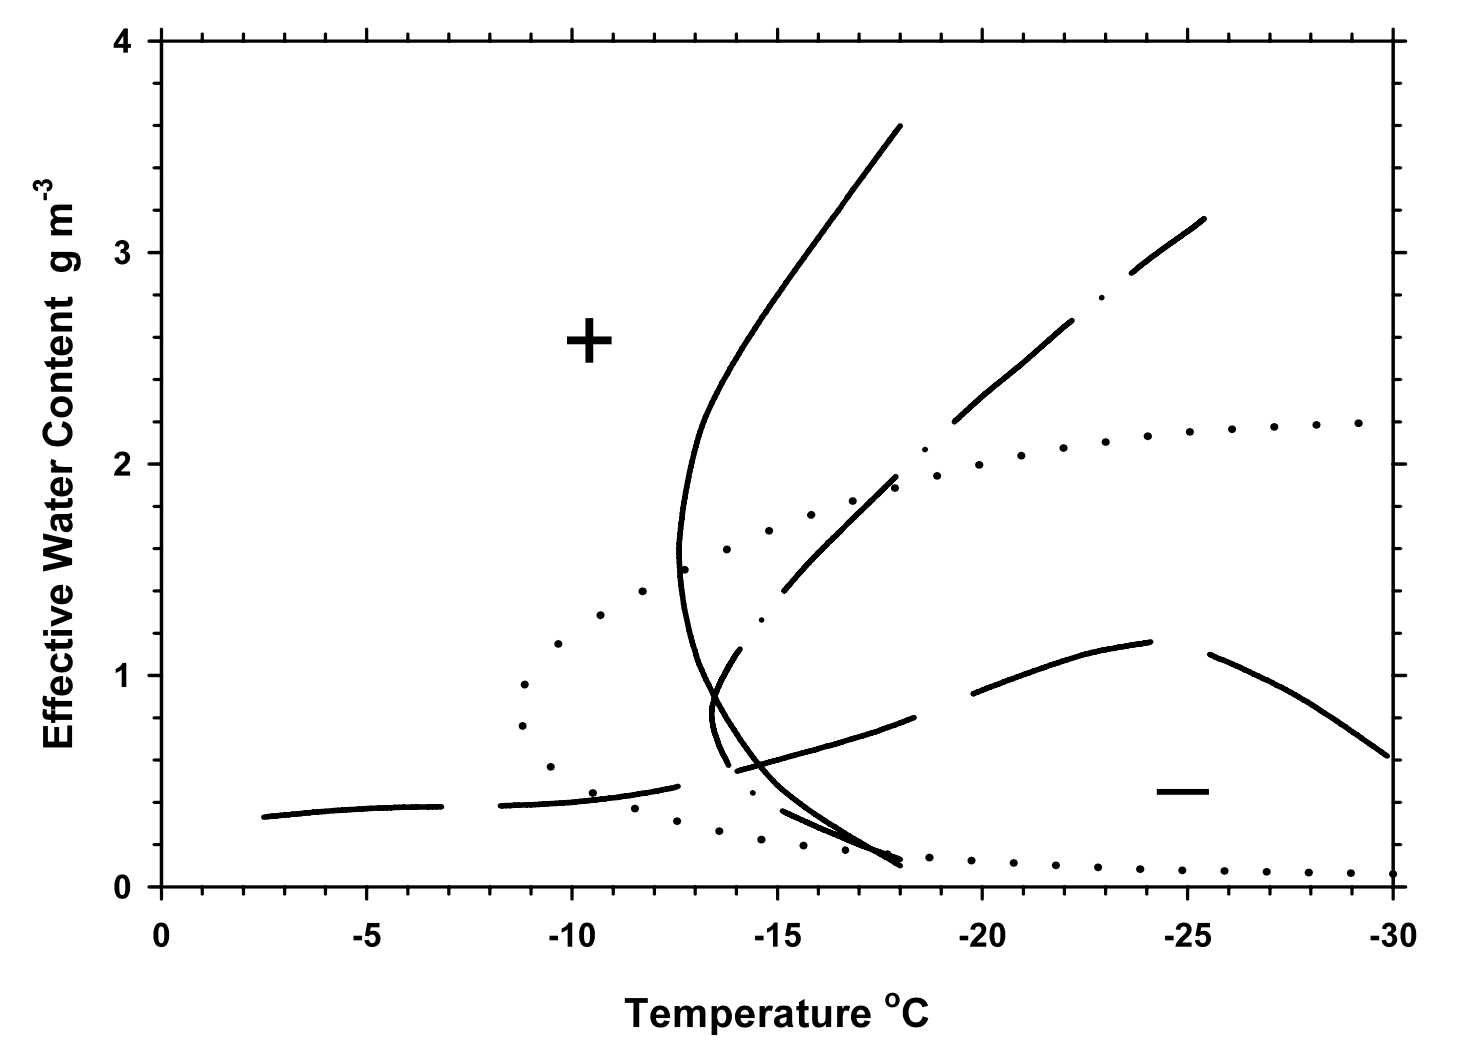
\includegraphics[width=0.7\textwidth]{charge_reverse_curves}
% \caption{\textit{Lab results}}
\caption{\textit{Lab results}}
% \vspace{-50pt}
\label{fig:charge_reverse_curves}
\end{figure}

\begin{figure}[H]
% \clearpage
\centering
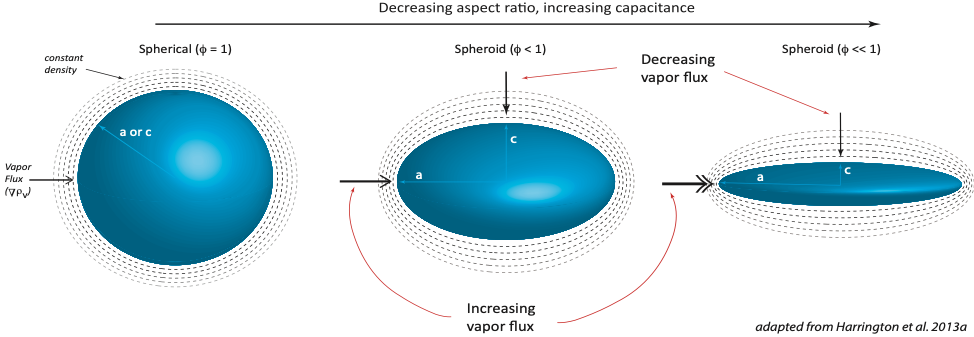
\includegraphics[width=\textwidth]{IceHabbit}
\caption{\textit{Evolution of ice aspect ratio as represented by spheroids. As aspect ratio evolves away from spherical, vapor density gradients concentrate over the area of greatest curvature. Based on Figure 2 in Harrington et al. (2013a).}}
\label{fig:icehabit}
\end{figure}

\end{document}
